\documentclass{ctexart}
\usepackage{graphicx}
\usepackage{caption}
\usepackage{float}
\usepackage{amsmath}
\usepackage{fancyhdr}
\usepackage{xunicode-addon}
\usepackage{booktabs}
\usepackage[a4paper,hmargin=1.25in,vmargin=1in]{geometry}
% !TeX program = xelatex
\title{\begin{figure}[H]
	\centering 
	\includegraphics[height=7cm,width=14cm]{E:/Pictures/中科大.jpg}
	\end{figure}\Huge\textbf{Lab 6}\\\huge{}}
\date{}
\punctstyle{banjiao} 
\pagestyle{fancy}
	\fancyhead[C]{\LARGE\textbf{Lab 6}}
	\fancyhead[L]{}
	\fancyhead[R]{}
	\fancyfoot[C]{\thepage}
\begin{document}
	\maketitle
	\thispagestyle{empty}
	
	\[\makebox{\Large{姓名:\underline{\makebox[5cm]{高茂航}}}}\]
	
    \[\makebox{\Large{学号:\underline{\makebox[5cm]{PB22061161}}}}\]
	
	$$\makebox{\Large{日期:\underline{\makebox[5cm]{2024.6.10}}}}$$
	
	\clearpage

	\pagenumbering{arabic}
	\section{Problem Descriptions}

	\section{Analysis and Algorithms} 
	\subsection{Algorithm 1 FFT}

$n\leftarrow length[f]$ 

$\textbf{if }n= = 1$

$\quad\quad\textbf{then return }f$

$\textbf{end if}$

$\omega_n\leftarrow e^{\boldsymbol{i}2\pi/n}$

$\omega\leftarrow1$

$\mathbf{f}^{0}\leftarrow(f_{0},f_{2},\ldots,f_{n-2})$

$\mathbf{f}^{1}\leftarrow(f_{1},f_{3},\ldots,f_{n-1})$

$\mathbf{g}^0\leftarrow$FFT$(\mathbf{f}^0)$

$\mathbf{g}^1\leftarrow$FFT$(\mathbf{f}^1)$ 

$\textbf{for }k\leftarrow 0$ to $n/ 2- 1\textbf{do}$

$\quad\quad\mathbf{g_k}\leftarrow\mathbf{g}_k^0+\omega\mathbf{g}_k^1$

$\quad\quad\mathbf{g_{k+n/2}}\leftarrow\mathbf{g}_k^0-\omega\mathbf{g}_k^1$

$\quad\quad\omega\leftarrow\omega\omega_n$

\textbf{end for}

\textbf{return g}
	\subsection{Algorithm 2 IFFT}
	\subsubsection{方法1}

$n\leftarrow length[f]$ 

$\textbf{if }n= = 1$

$\quad\quad\textbf{then return }f$

$\textbf{end if}$

$\omega_n\leftarrow e^{\boldsymbol{-i}2\pi/n}$

$\omega\leftarrow1$

$\mathbf{f}^{0}\leftarrow(f_{0},f_{2},\ldots,f_{n-2})$

$\mathbf{f}^{1}\leftarrow(f_{1},f_{3},\ldots,f_{n-1})$

$\mathbf{g}^0\leftarrow$IFFT$(\mathbf{f}^0)$

$\mathbf{g}^1\leftarrow$IFFT$(\mathbf{f}^1)$ 

$\textbf{for }k\leftarrow 0$ to $n/ 2- 1\textbf{do}$

$\quad\quad\mathbf{g_k}\leftarrow\mathbf{g}_k^0+\omega\mathbf{g}_k^1$

$\quad\quad\mathbf{g_{k+n/2}}\leftarrow\mathbf{g}_k^0-\omega\mathbf{g}_k^1$

$\quad\quad\omega\leftarrow\omega\omega_n$

\textbf{end for}

$\mathbf{g} = \mathbf{g}/2$

\textbf{return g}
\subsubsection{方法2}
$\mathbf{f_{temp}}\leftarrow(f_{0},f_{n-1},f_{n-2}\ldots,f_{2})$

$\mathbf{g}\leftarrow$FFT$(\mathbf{f_{temp}})$

$\mathbf{g} = \mathbf{g}/n$

$\textbf{return g}$
	\section{Results}
	\begin{figure}[H]
		\centering 
		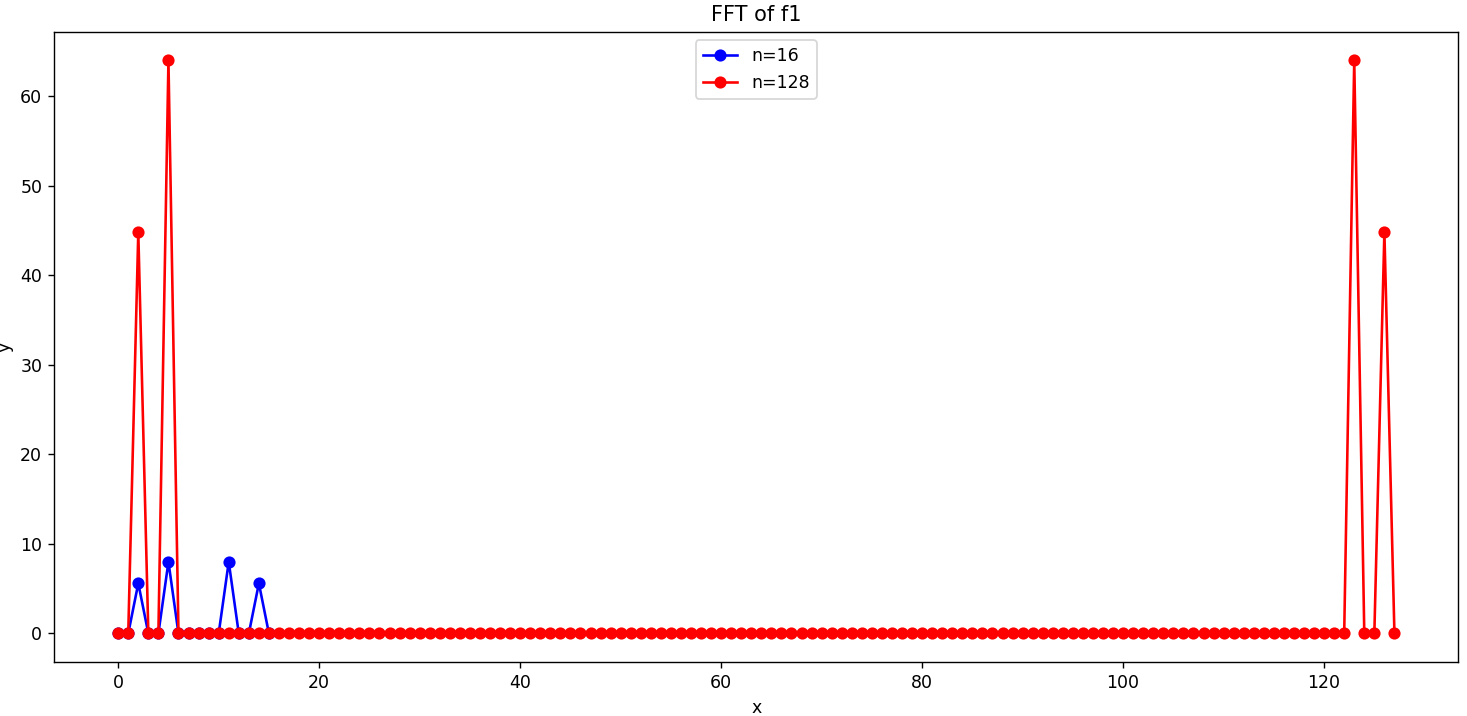
\includegraphics[height=7cm,width=14cm]{1.png}
		\end{figure}
		
			\begin{figure}[H]
				\centering 
				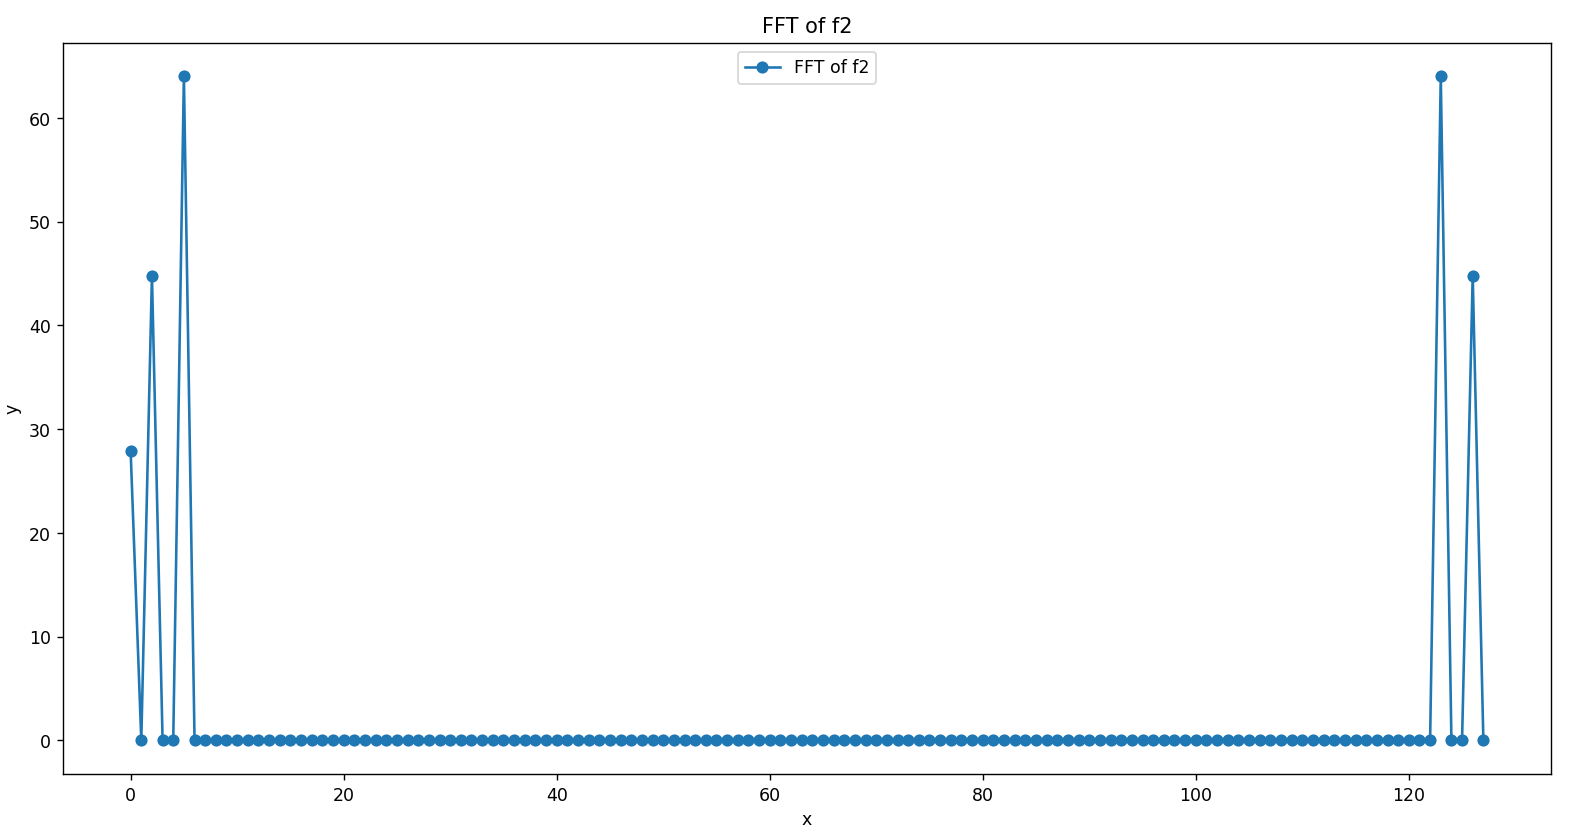
\includegraphics[height=7cm,width=14cm]{2.png}
				\end{figure}
				\begin{figure}[H]
					\centering 
					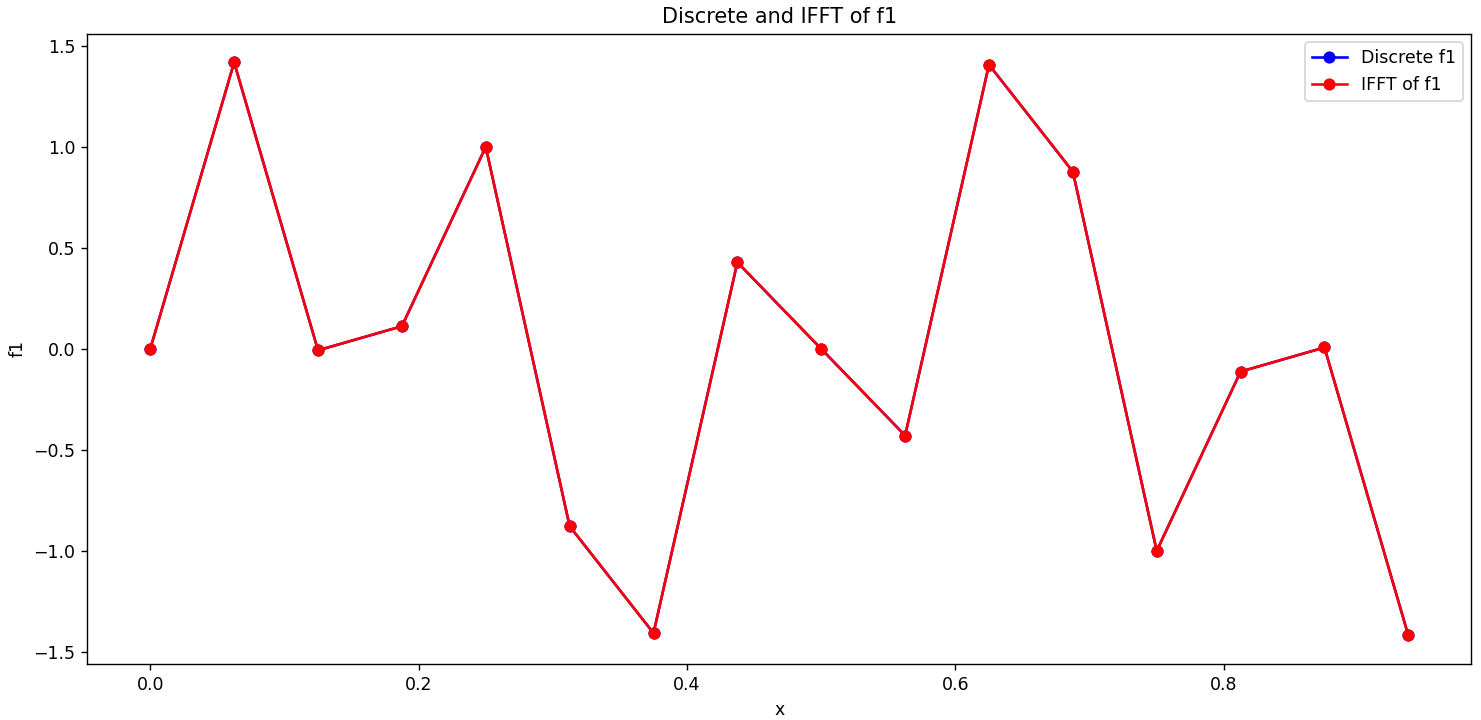
\includegraphics[height=7cm,width=14cm]{3.png}
					\end{figure}
					\begin{figure}[H]
						\centering 
						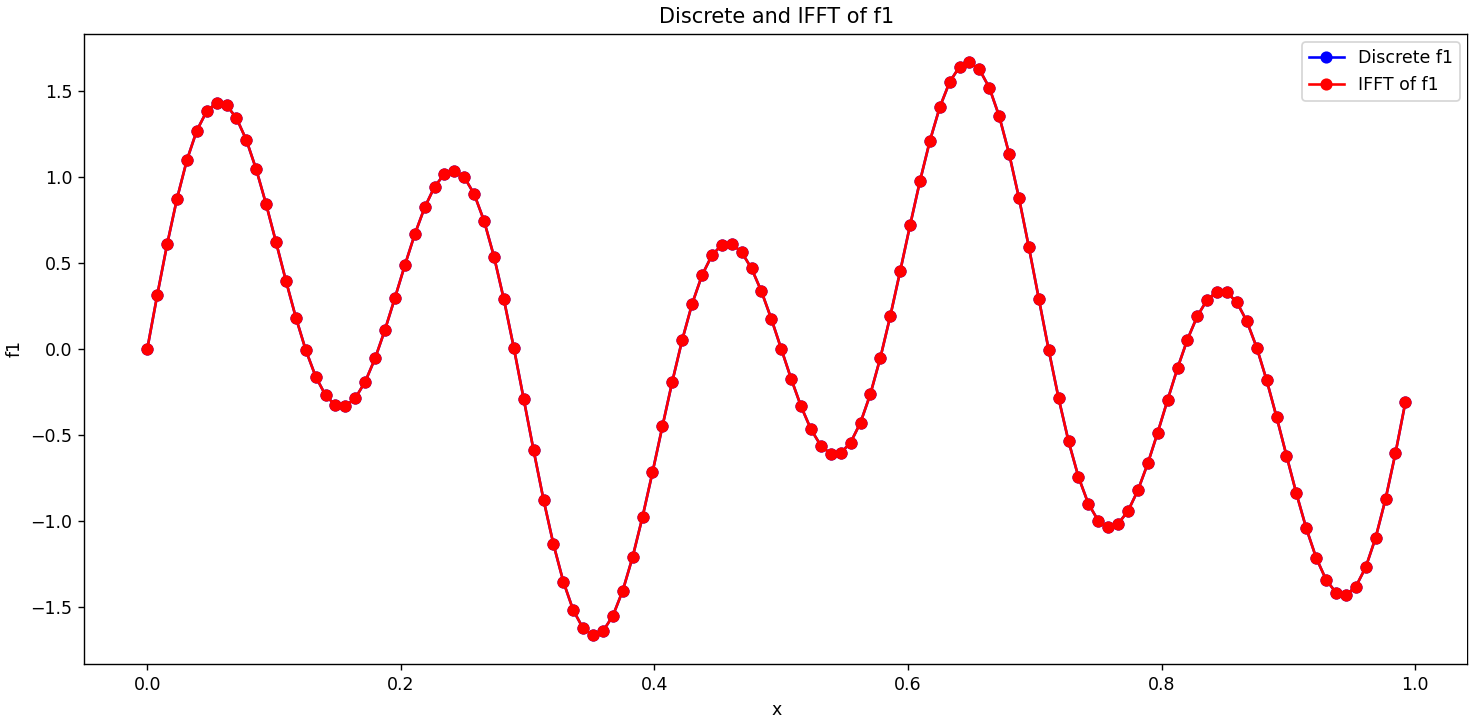
\includegraphics[height=7cm,width=14cm]{4.png}
						\end{figure}
						\begin{figure}[H]
							\centering 
							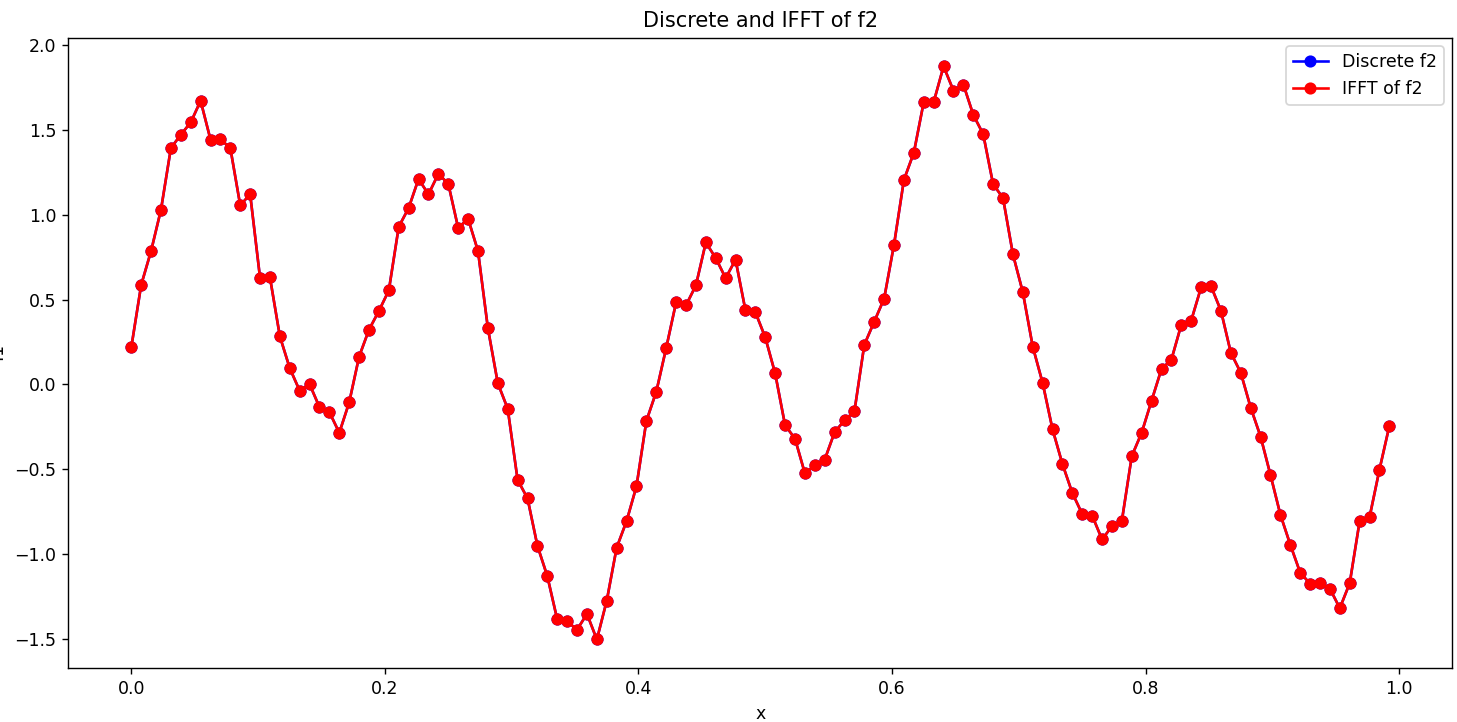
\includegraphics[height=7cm,width=14cm]{5.png}
							\end{figure}
							\begin{figure}[H]
								\centering 
								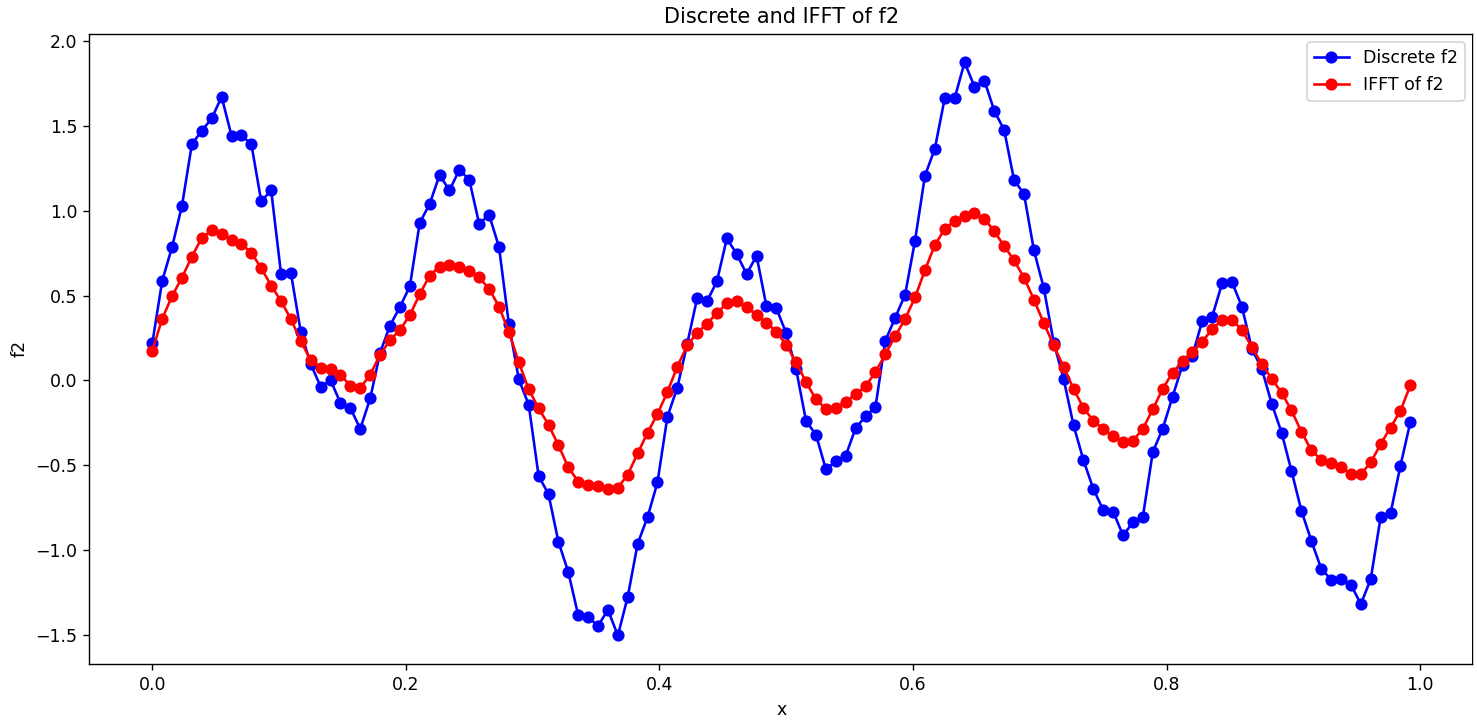
\includegraphics[height=7cm,width=14cm]{6.png}
								\end{figure}
		\section{Conclusion}
    \end{document}